Our approach is based on the following observations.
\begin{itemize}
\item In a well-designed web application targeted for PaaS environments, 
most of the ``work'' is done by
curated services intrinsic to the PaaS cloud~\cite{Jayathilaka:2015:RTS:2806777.2806842}.
%Put
%another way, if the application is not leveraging the PaaS services to the
%fullest extent, it is not taking advantage of the PaaS model.
\item An application making maximal use of the PaaS services finds that its
performance is defined by the performance of these services.  Since the 
implementation and deployment details of the PaaS services are hidden
from the applications,
performance diagnostics must also be implemented as an intrinsic PaaS service.
\item The integrity and accuracy of application performance diagnostics
cannot rely on programmer-introduced application instrumentation.
\end{itemize}
Thus, the key intuition behind Roots is that as a curated PaaS service
it has visibility into all the activities that occur in various layers of the cloud,
including all invocations of the PaaS kernel services made by the applications.

%Therefore it can automatically collect
% data regarding events that are related to application request processing. 
%The cloud platform can then analyze the collected data offline (but in near realtime) to detect 
%performance anomalies and identify root causes.
%
%We argue that data collection can be implemented efficiently in the cloud platform so as to not
%introduce a significant overhead to deployed applications.
%Moreover, data collection can be always active in the cloud thus relieving the application developers
%from having to instrument their code, or setting up external monitoring.
%The data analysis can benefit from the vast amount of compute
%resources available in the cloud platform. The offline processing ensures that request
%latency is not impacted by monitoring, and the near realtime analysis ensures that developers
%and other interested parties are notified of performance anomalies urgently. 

\subsection{Data Collection and Correlation}

Since Roots does not rely on application instrumentation inserted by the
programmer or third-party tools, it must infer application performance traits from 
the performance of the PaaS services in the cloud platform. 
Typically, each individual layer of the cloud platform collects data regarding
its own state changes facilitating measurement of the time taken in service
operations. However, a layer cannot monitor state changes
in other layers without violating software isolation properties of
layering in general.   That is, layers typically log their own internal
activities, but do not (or cannot) correlate these activities
with the internal activities of other layers.
 
%There are two issues that need to be addressed when designing a monitoring framework for
%a system as complex as a PaaS cloud.
%\begin{enumerate}
%\item Collecting data from multiple different layers.
%\item Correlating data collected from different layers.
%\end{enumerate}

%However,
%processing an application request involves cooperation of multiple 
%layers. For example, an application request gets routed through the front-end server before
%it reaches the application server. The application server may then invoke one or more PaaS kernel
%services. Depending on how the kernel services are implemented,
%even more layers may get involved in processing the request. 
%In order to facilitate systemwide monitoring and
%bottleneck identification, we should be able to gather data from all the different layers involved
%in processing a request. Then we should be able to correlate the collected data, and tie the events that
%are related to the same request together.

Roots modifies the front-end request server (typically a software load balancer) 
to tag all incoming application requests with unique identifiers. Doing so enables Roots
to associate invocations of PaaS kernel services with a particular request, and by extension with an application.
This request identifier is attached to an HTTP request as a header, which is visible to all 
internal components of the PaaS cloud. We configure performance data collecting
agents in each software layer in the PaaS 
cloud to record the request identifiers along with any events they capture. 
This way we maintain the relationship between application requests, and the resulting
local state changes in different layers of the cloud without breaking the existing level
of abstraction in the cloud architecture. 
To make this approach scalable, we collect events independently within their layers, and 
aggregate on-demand.

%
%This approach is also scalable, since the events are
%recorded in a distributed manner without having to maintain any state at the data collecting agents. 
%The data analysis components can later
%aggregate the recorded events by request identifiers to efficiently group the related events,
%in on demand fashion.
%
\begin{figure}
\centering
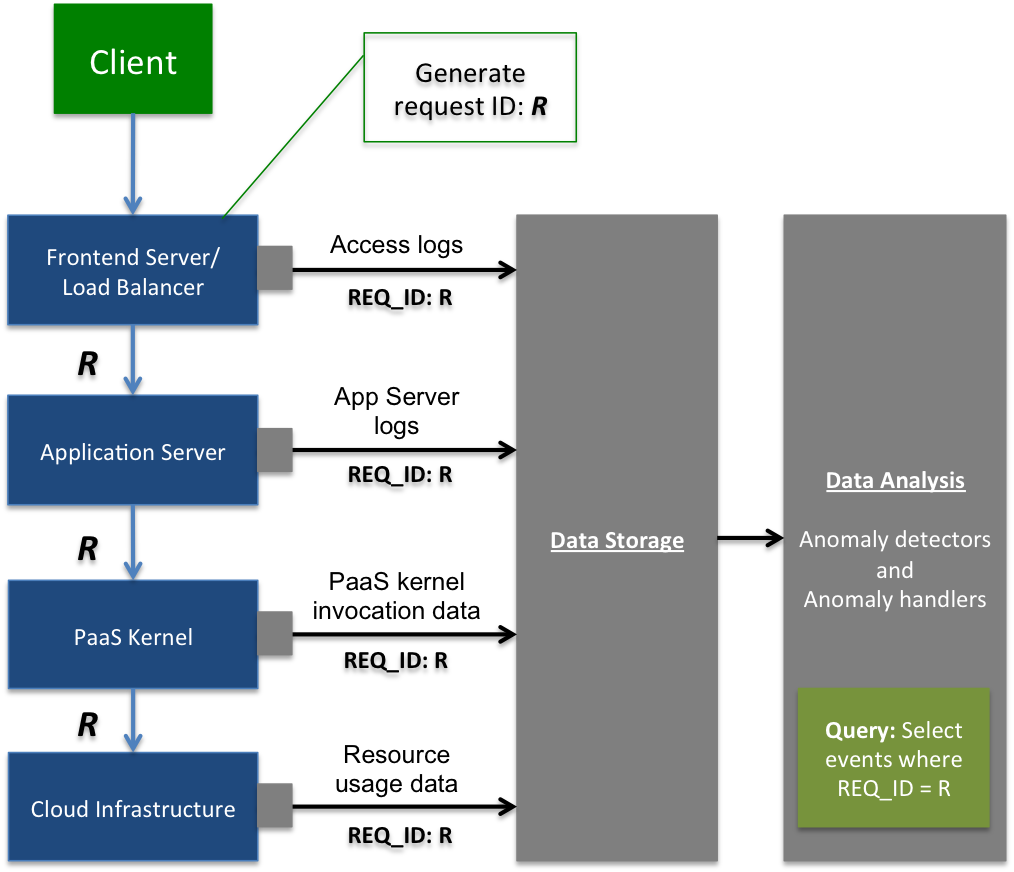
\includegraphics[scale=0.5]{apm_architecture}
\caption{Roots APM architecture.  Roots injects a request ID ($R$) at request
ingress that it uses to correlate events at each level of the stack.}
\label{fig:apm_architecture}
\end{figure}
%
%Figure~\ref{fig:apm_architecture} illustrates the high-level architecture of Roots, and how 
%it fits into the PaaS stack. APM components are shown in grey, with their interactions indicated
%by the black lines. The small grey boxes attached to the PaaS components represent the
%agents used to instrument the cloud platform for data collection purposes. 
%In the diagram a user request is getting tagged with the identifier value
%$R$ at the front-end server. This identifier is passed down to the lower layers of the cloud
%along with the request. Events that occur in the lower layers as a result of processing this request
%are recorded with the request identifier $R$, so we can correlate them later. For example, in the 
%data analysis component we can run a filter query to select all the events related to a particular
%request (as shown in the pseudo query in the diagram). Or we can run a ``group by'' 
%query to select all events, and aggregate them by the request identifier.

Figure~\ref{fig:apm_architecture} shows Roots collecting data from all
layers in a PaaS stack (i.e. full stack monitoring). 
Such monitoring enables us to trace the execution of individual requests
through the cloud platform. In addition
to the data collecting agents directly integrated with the cloud platform, Roots employs
a collection of application benchmarking processes that periodically measure
application latency. Roots uses measurements taken by these processes to
evaluate the performance SLOs of each application.

%Finally, at the lowest infrastructure level, we can collect information related to virtual machines, containers
%and their resource usage. We can also gather metrics on network usage by individual components which
%might be useful in a number of traffic engineering use cases. Where appropriate we can also scrape
%hypervisor and container manager logs to get an idea of how resources are allocated and released over
%time.

To avoid introducing delays to the application request processing flow, we implement
all Roots data collecting agents as asynchronous tasks. That is, none of them 
suspend application request processing to store data.
All expensive I/O tasks related to data collection and storage in Roots are
executed out of the request processing flow.
Roots aggregates all data into log files or memory buffers that are local to the components being
monitored. This locally collected (or buffered) data is periodically sent
to the data storage components of Roots using separate background tasks and batch communication
operations. We also isolate PaaS services from potential
failures in the Roots data collection or storage components to avoid cascading failures.

\subsection{Data Storage}

Roots data storage uses a database for persisting and querying monitoring data.
%Cloud providers have the freedom to implement this component in any way they see fit, as long
%as it scales to the number of applications deployed in the cloud platform. 
We index key properties (application and time intervals) to optimize query performance.
Roots also performs garbage collection for removal of 
old monitoring data when it is no longer useful 
to its anomaly detection algorithms. 

\subsection{Data Analysis}

Roots data analysis component uses two basic abstractions: \textit{anomaly detectors} 
and \textit{anomaly handlers}.
Anomaly detectors are processes that periodically analyze the data collected for
each deployed application. Roots supports multiple detector implementations, where each implementation
uses a different statistical method to look for performance anomalies. Detectors are configured
per-application, making it possible for different applications to use different anomaly 
detectors. Roots also supports multiple concurrent anomaly detectors on the same application, which can be used
to evaluate the efficiency of different detection strategies for any given application. Each
anomaly detector has an execution schedule (e.g. run every 60 seconds), and a sliding window 
(e.g. from 10 minutes ago to now)
associated with it. The boundaries of the window determines the time range
of the data processed by the detector at any round of execution. Window is updated 
after each round of execution. 
%Our anomaly detector abstraction is general
%enough to support detecting a wide range of anomalies. However, in our work we
%mainly focus on anomaly detectors that check for violations of performance SLOs.

When an anomaly detector finds an anomaly in application performance, it sends an event
to a collection of anomaly handlers. The event consists of a unique anomaly identifier, 
timestamp, application identifier, and the source detector's sliding window corresponding to the
anomaly. Anomaly handlers are configured globally (i.e. each handler
receives events from all detectors), but each handler can be configured to handle only
certain types of events. Furthermore, handlers can fire their own events, which are also delivered to
all listening anomaly handlers. Similar to detectors, Roots supports multiple anomaly handlers
that support logging, alerting, dashboard updating, 
workload change detection, and bottleneck identification.

%Roots also includes two special anomaly handlers:
%a workload change analyzer, and a bottleneck identifier.
%Moreover, it uses shared memory for fast communication 
%communication between detectors and handlers.

%The ability of anomaly handlers to fire their own events, coupled with their support
%for responding to a filtered subset of incoming events enables constructing
%elaborate event flows with sophisticated logic. For example, the workload
%change analyzer can run some analysis upon receiving an anomaly event
%from any anomaly detector. If an anomaly cannot be associated with a workload
%change, it can fire a different type of event. The bottleneck identifier, can
%be programmed to only execute its analysis upon receiving this second type of event.
%This way we perform the workload change analysis first, and perform the
%systemwide bottleneck identification only when it is required to do so.

%Both the anomaly detectors and anomaly handlers work with fixed-sized sliding windows.
%They can discard any old data as the sliding window moves along the time line.
%Therefore the amount of state information these entities must keep in memory has
%a strict upper bound. 
%The extensibility of Roots is primarily achieved through the abstractions of anomaly
%detectors and handlers. Roots makes it simple to implement new detectors and handlers,
%and plug them into the system. Both the detectors and the handlers are executed
%as lightweight processes that do not interfere with the rest of the processes in
%the cloud platform. Failures in detectors and handlers have no impact
%on the cloud platform or the deployed applications.

\subsection{Roots Pods}
\label{sec:process_mgt}

%\begin{figure}
%\centering
%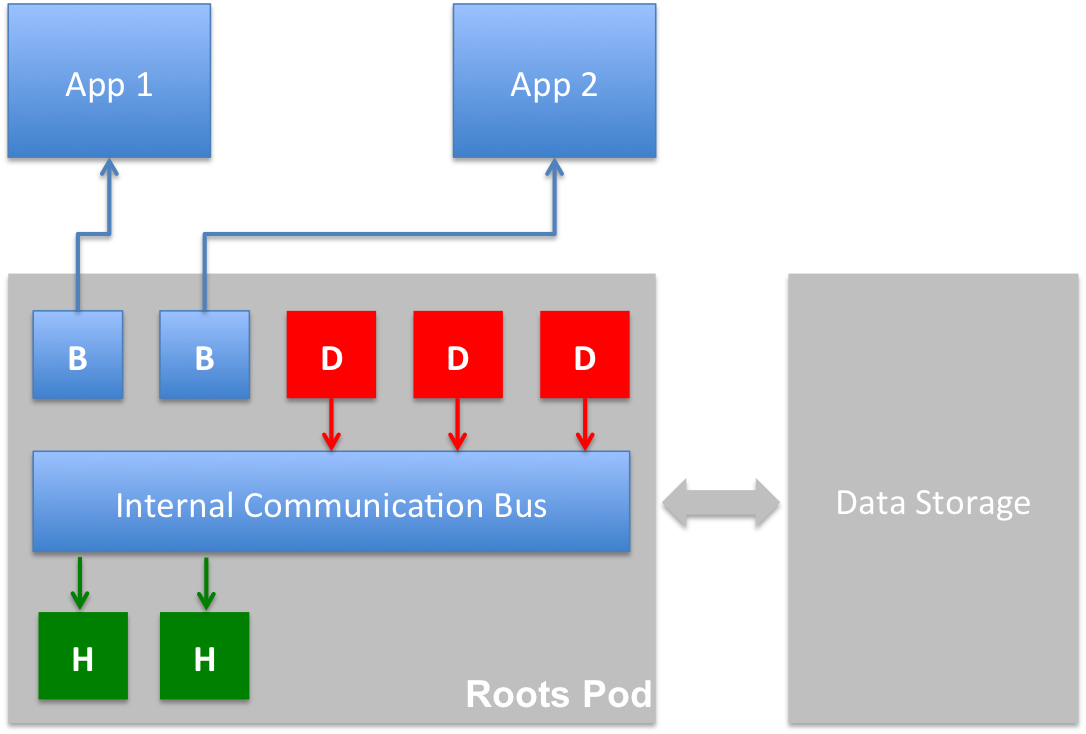
\includegraphics[scale=0.4]{roots_pod}
%\caption{Anatomy of a Roots pod. The diagram shows 2 application benchmarking processes (B), 
%3 anomaly detectors (D), and 2 handlers (H).}
%\label{fig:roots_pod}
%\end{figure}
%Most data collection activities in Roots can be treated as passive -- i.e. they
%happen automatically as the applications receive and process requests in the cloud
%platform. They do not require explicit scheduling or management. In contrast,
%application benchmarking and data analysis are active processes that require
%explicit scheduling and management.  This is achieved by 

Roots groups data analysis processes (i.e. anomaly detectors and handlers), 
and application benchmarking processes into units called \textit{Roots pods}. 
Each Roots pod is responsible for starting and maintaining a collection of
benchmarkers and data analysis processes. 
%Each of these processes are light enough, so as to pack a large number of them
%into a single pod. 
Pods are self-contained entities, and there is no inter-communication
between pods. 
Processes within a pod communicate via 
shared memory, and call out to Roots data storage to retrieve 
performance measurements for analysis. Such encapsulation facilitates 
efficient starting/stopping of pods 
without impacting other PaaS and Roots components. Our pods design also facilitates
replication for high availability and application load distribution
among multiple pods for scalability.
%Figure~\ref{fig:roots_pod} illustrates a Roots pod monitoring two applications.
%The anomaly detectors and handlers communicate
%using an internal shared memory communication bus, so that events triggered by one anomaly
%detector flow into all handlers. 

%To automate the process of managing pods, they can be tied into the core
%process management framework of the PaaS cloud. That way whenever the cloud
%platform initializes, a collection of pods can be started automatically.
%Application deployment process of the PaaS cloud can be augmented
%to register each new application with one of the available pods, so that the
%benchmarkers and anomaly detectors can start running on the application.
%Moreover, pods can be moved around or restarted as needed in response
%to errors and autoscaling events that occur in the cloud platform.
